%!TEX root = main.tex

\section{Introduction}
\label{sec:introduction}

The industrial adoption of microservices has led to increasingly complex configuration schemes that are manually fine-tuned by engineers. Ganek and Corbi discussed the need for autonomic computing to handle the complexity of managing software systems~\cite{ganek_dawning_2003}. They noted that managing complex systems has become too costly, prone to error, and labour-intensive because pressured engineers make mistakes, increasing the potential of system outages with a concurrent impact on business. This has driven many researchers to study self-adaptive systems (e.g., \cite{porter_rex:_2016, andrew_pavlo_self-driving_2017, salehie_self-adaptive_2009, ganapathi_predicting_2009, herbst_self-adaptive_2014, faniyi_architecting_2014}); however, the software industry still lacks practical tools to provide self-adaptive system configurations. Thus, most system configuration and tuning is performed manually, often at runtime, which is known to be a very time consuming and risky practice \cite{ganek_dawning_2003, using_prob_reasoning_automate_software_tuning, de_lemos_software_2013}.

In this work we present \projectname{}, a tool that enables engineers to integrate self-adaptation mechanisms into their systems. \projectname{} delegates the configuration and tuning of a system to a learned model, rather than requiring engineers to perform these operations manually or through manually tuned heuristics.

Building self-adaptive systems is a major engineering challenge \cite{brun_engineering_2009}. \projectname{}'s proposal is to enable self-adaptation by giving the user the ability to inject the main components of a self-adaptive mechanism into an existing target system in a loosely-coupled fashion.

\begin{figure}[!htb]
	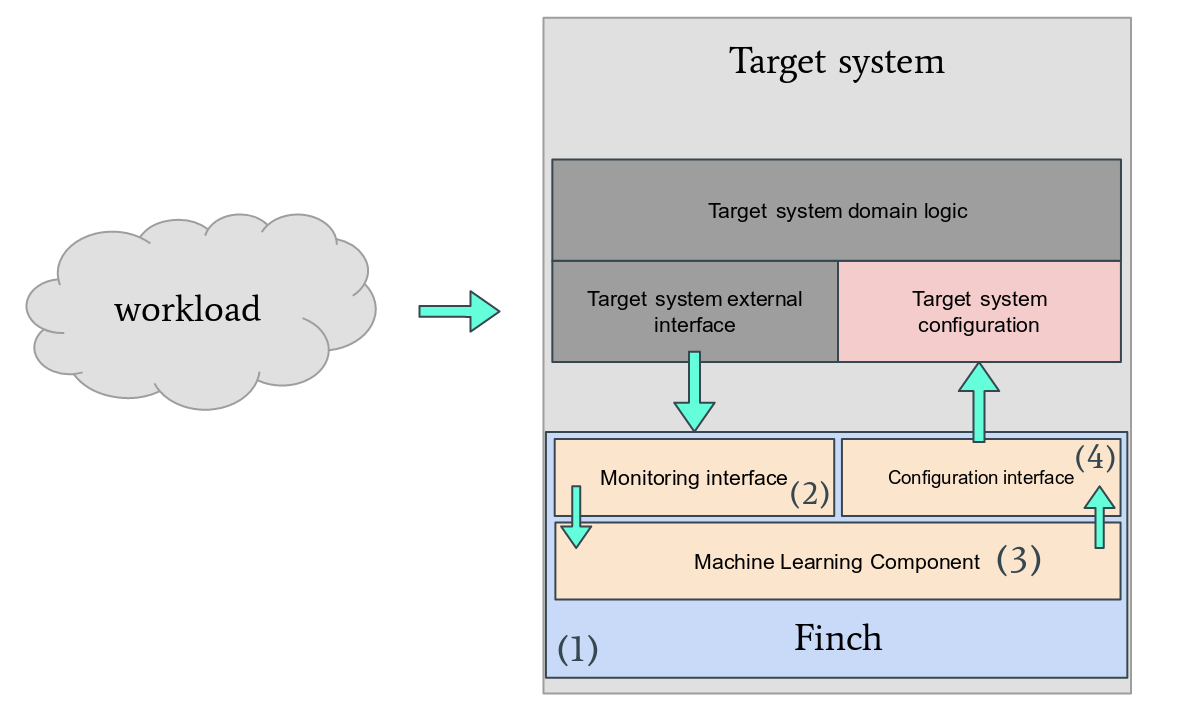
\includegraphics[scale=0.2]{images/finch.png}
  \caption{How finch integrates into a target system; (1) Finch is injected into the target system, (2) it Monitors and analyzes the target system’s context, (3)Finch learns how to configure the target systems, (4) Interface executes configuration adaptation plans, adapting the target system.
}
  \label{fig:finch}  
\end{figure}

One of \projectname{}'s main goals is to provide self-adaptive configuration support with minimal engineer effort. \projectname{} uses ideas from self-adaptive systems, system observability, machine learning, and control theory to automatically asses the system's environment, predict the impact of changes that could potentially improve the system, and make these changes automatically.

My approach consists of providing mechanisms for injecting a control loop into an existing target system through an API for collecting relevant system metrics and configurations as the system executes. The user maps Service Level Agreements (SLAs) to a subset of these metrics, feed them into a machine learning component that is concurrently relearning the model while analyzing current event data which then predicts optimal configurations for the system for its given context. As a result, \projectname{} provides adaptation plans that can be both \emph{automatically executed}, allowing the system to have self-adaptive capabilities, and \emph{interpretable}, allowing engineers to understand the impact of a change in the configuration space before it is deployed.

The main contributions of this paper are:

\begin{itemize}
  \item A methodology for assisting the development and evolution of self-adaptive systems, regardless of the presence of self-adaptability in the system's foundations. Such methodology is encapsulated in \projectname{}.
  \item Demonstrating how minimal changes to the system can support this approach, and how Service-Level Agreements can be modeled and mapped to optimization objectives.
  \item A group of experiments to evaluate \projectname{}'s performance when integrated into a web service, demonstrating how \projectname{} can learn how to configure it and improve its performance while incurring 8.5\% of performance overhead.
\end{itemize}

Chapter 2 discusses past research in the space of self-adaptive systems and provides fundamental background for our approach. Chapter 3 outlines the design and usage of \projectname{}, explaining the blend of ideas from different fields that lead to its principle design decisions. Chapter 4 describes \projectname{} and its implementation. Chapter 5 presents the evaluation performed on \projectname{}, followed by a discussion on limitations and future directions in Section 6.

%
% here we reorganize these characteristics into the following terminology:

% \begin{itemize}
%   \item \textbf{Self-Awareness}: an autonomic system needs to know itself;
%   \item \textbf{Self-configuring}: an autonomic system must configure and reconfigure itself under varying and unpredictable conditions;
%   \item \textbf{Self-optimization}: an autonomic system never settles for the status quo, it always looks for ways to optimize its workings, it will anticipate the optimized resources needed to meet a user's information needs while keeping its complexity hidden;
%   \item \textbf{Self-healing}: An autonomic system must perform something akin to healing, it must be able to recover from routine and extraordinary events that might cause some parts to malfunction.
% \end{itemize}


% \begin{itemize}
%   \item Use of system observability to collect a sufficiently big time series dataset that represents the state of a system and its components in relation to time;
%   \item Use of Machine Learning applied to time series data to analyze and predict workload and optimal configuration in order to provide adaptation plans;
%   \item Use of Online Learning to provide constant relearning of the model to adapt to different scenarios and requirements;
%   \item Use of Service Level Objectives as a way to define the system's performance goals that will be used by the tool as optimization objectives;
%   \item Use of the concepts in control theory as the central component of this tool, in which it implements a variation of the well known and studies MAPE loop (Monitor, Analyze, Plan, Execute);
%   \item Abstraction of all the concepts above into a tool that can be integrated to compatible systems, including systems that were built without self-adaptation in mind. 
% \end{itemize}

% The rest of the paper is structure as following: 


% I can develop a bit more on this by using this survey's result: According to a recent
% IT resource survey by the Merit Project of Computer Associates International, 1867 respondents grouped the most common causes of outages into four areas of data center operations: systems, networks, database, and applications.
% Most frequently cited outages included:
%- For systems: operational error, user error, third-party software error, internally %developed software problem, inadequate change control, lack of automated processes
%- For networks: performance overload, peak load problems, insufficient bandwidth
%- For database: out of disk space, log file full, performance overload
%- For  applications:  application  error,  inadequate change control, operational %error, nonautomated application exceptions
% A nice point is that these are the problems we're still facing whenever we deal poorly with the complexity of the systems

% It would be nice also to cite IBM autonomic computing initiative

% IBM’s autonomic computing initiative has been outlined broadly. Paul Horn described this “grand challenge” and called for industry-wide collaboration toward developing autonomic computing systems that have characteristics as follows: ● To be autonomic  a system needs to “ know itself ”— and consist of components that also possess a sys- tem identity. ● An autonomic system must con fi gure and recon- fi gure itself under varying and unpredictable con- ditions. ● An autonomic system never settles for the status quo — it always looks for ways to optimize its work- ings. ● An autonomic system must perform something akin to healing — it must be able to recover from routine and extraordinary events that might cause some parts to malfunction. ● A virtual world is no less dangerous than the phys- ical one, so an autonomic computing system must be an expert in self-protection. ● An autonomic computing system knows its envi- ronment and the context surrounding its activity, and acts accordingly. ● An autonomic system cannot exist in a hermetic environment (and must adhere to open standards). ● Perhaps most critical for the user, an autonomic computing system will anticipate the optimized re- sources needed to meet a user ’ s information needs while keeping its complexity hidden.

\section{Related work and foundations}
\label{sec:rw}

\projectname{} draws ideas from many different, although overlapping, fields. Here we discuss where these ideas come from and how they relate to \projectname{}.

\textcolor{blue}{}

% Explanation for related work scheme: control theory, SE and mape-k => time series => ts for resources allocation => best ts forecasting approaches => workload simulation => hogna: almost what I wanted but not quite. plus: flawed => continuing on hogna: here's what didn't work and the differences => previous work are reactive, where's aot mape-k => peloton: like that but generic

% note: it would be better to focus on ml applied to system, control theory + self-adapative community seems very fancy and annoying
\subsection{Control theory in software engineering}

The ideas in control theory have been widely adopted in the software engineering research community, with special attention to the Monitor-Analyze-Plan-Execute over a shared Knowledge, known as MAPE-K feedback loop, which proved to be a powerful tool to build self-adaptive systems \cite{arcaini_modeling_2015, salehie_self-adaptive_2009, Brun2013, computing_architectural_2006, kephart_vision_2003, de_lemos_software_2013}. Angelopoulos et al discussed the intersection between software engineering and control theory \cite{filieri2015software}. They showed how control-theoretical software systems are implemented and their design process, as well as the differences of the word ``adaptation'' in both fields. All These works were shown to be invaluable to the development of \projectname{}, because the injection of a MAPE-K loop into the target system is the core component of \projectname{}.

\subsection{Machine learning in control theory}

The applications of machine learning in control theoretical models have been discussed in \cite{Gillula10_FusingMachineLearningControlTheory}, where the main idea is to take advantage of high performance of machine learning methods while using control theory to guarantee safety and controllability. Reinforcement learning \cite{Sutton:1998:IRL:551283} has similar goals to those in control theory, but with different approaches. \projectname{} uses ideas from machine learning, reinforcement learning, and control theory to enable self-adaptability. Thus, instead of hard-coding configuration heuristics in a system, the control theory aspect of \projectname{} (the MAPE-K loop) uses machine learning techniques to learn patterns in the target system and make fast predictions in order to create adaptation plans.

\subsection{Time series analysis}

Time series data has been used to analyze and predict patterns in data with respect to time, with applications on understanding how to efficiently allocate computational resources, which is a key strategy in our work to provide ahead-of-time adaptation.

Between 2007 and 2011, many techniques for forecasting workload and performance metrics using time series data have been realized \cite{gmach2007workload, towards_autonomic_allocation, bobroff2007dynamic, meng2010efficient, caron2011pattern}. With these forecasts, these authors provided methodologies for virtual machine allocation in data centres. These works did not focus on tools for applying machine learning to software systems nor on tools to enable self-adaptability in arbitrary software systems---which is our end goal.

Herbst et al. contributed with a survey of state-of-the-art forecasting approaches based on time series analysis and a decision-based technique to select the best forecasting method based on user-specified objectives \cite{herbst_self-adaptive_2014}. They provided a useful technique to reliably forecast workload and performance metrics based on time series analysis, which is an important component in our tool. To enable self-adaptation in a system is to first understand the patterns in its context over time. In \projectname{} we use these ideas and techniques to forecast workloads that, with the current configuration, could lead to SLA violations. Thus, enabling \projectname{} to create an adaptation plan for this forecast and schedule the adaptation carry out.

\subsection{Workload modelling}

Another important aspect of \projectname{} is being able to simulate workload intensity for initial training of the adaptation model. To have an accurate workloads, we need to model them as closely as possible to real-world workloads. Herbst et al. presented the Descartes Load Intensity Model \cite{kistowski_modeling_2017}, a powerful tool for describing load intensity variations over time, that can also be used for an accurate benchmarking based on realistic workload and performance analysis. \projectname{} uses some of these ideas to model and simulate workloads for training the adaptation model.

\subsection{Self-adaptive systems}

Cornel Barna et al proposed Hogna, a platform for deploying self-adaptive applications in cloud environments \cite{barna_hogna:_2015}. Hogna provides a framework that abstracts deployment details, for example: spinning-off and managing instances on Amazon EC2 or OpenStack, enabling the user to focus on the adaptation mechanism. A key difference between Hogna and \projectname{} is that \projectname{} is not a deployment framework, but rather a library that assists the implementation of a MAPE-K closed loop by abstracting formal modelling to a machine learning model that can be matched with the specified SLAs, instrumented data, and identified configuration parameters of the system.

\projectname{} can be used either for managing adaptive deployment schemes or optimizing finer-grained knobs of a system, for instance, optimizing configuration knobs of a Postgres instance used by a system in order to improve performance and prevent SLO violations---which is our case study in this paper. In addition to that, a minor difference between these two tools is how much is asked from the user; Hogna asks for a configuration file that describes the topology to be deployed, monitors to use, and more related settings, custom java classes to handle specific behaviours, and PXL file with the model description and a configuration file for Kalman filters, whereas \projectname{} requires fewer actions from the user, while enabling self-adaptability and giving flexibility to the user: it can be used both for higher level tasks---deployment---and lower level tasks---self-tuning and self-configuring of smaller pieces of software.

Most previous work approaches the adaptation problem with reactive strategies: when a violation occurs---the service gets slower, errors are thrown---an adaptation is triggered and executed, stabilizing the system. \projectname{} is capable of providing the same style adaptation, while providing ahead-of-time adaptation: we use time-series analysis to create an adaptation plan for a future time, executing it right before a violation occurs, mitigating the risk of a potential SLO violation. 

Andrew Pavlo et. al. presented Peloton, a database system designed for autonomous operation~\cite{andrew_pavlo_self-driving_2017}. Similar to \projectname{}, one of their main goals was to decrease the need for manually-performed operations, though they focused solely on applying their ideas and techniques to their DBMS implementation. They achieved this by classifying the workload trends, collecting monitoring data, and forecasting resource utilization, then training a model based on this data to predict the best optimization plan. These ideas are important to our work, the key difference is that instead of directly embedding these ideas in a specific system---in this case a DBMS---and requiring the autonomous components to be tightly coupled to the system being configured, we are embedding a subset of these ideas in a tool that can be integrated in any arbitrarily chosen software system.

\subsection{Machine learning-enhanced software systems}

In a recent work entitled The Case for Learned Index Structures, Kraska et. al. have demonstrated that machine learned models have the potential to provide significant benefits over state-of-the-art database indexes~\cite{kraska_case_2017}. This research showed that by replacing manually tuned heuristics with learned models enabled it to outperform cache-optimized B-Trees by up to 70\%.

We draw much of our inspiration from this work; \projectname{}'s central idea is to allow systems that relies heavily on manual configurations and heuristics to be enhanced with learned models. This could be applied to many different domains. In this work we apply this idea to a REST-based API backend.

The idea of machine learning-enhanced software systems is to move from using the same algorithms, heuristics, data structures, or configurations in multiple different contexts, to personalized configurations; different configurations that perform better for different scenarios. This relates well to the No Free Lunch theorem:
\begin{quote}
  If an algorithm performs well on a certain class of problems then it necessarily pays for that with degraded performance on the set of all remaining problems.
\end{quote}

This is the main idea behind \projectname{}: the integration of learned models to generate adaptation plans according to the different scenarios.

\section{Design and Usage}
\label{sec:approach}

% This is a very important section, try to make it as clear as possible, the current version is not clear, it's just a brain dump. You can understand it because you see the end goal and the design, the readers do not

To integrate \projectname{} into the target system, the user has to do the following:
 
\begin{itemize}
  \item Instrument the target system
  \item Identify relevant configuration parameters for \projectname{}
  \item Define Service Level Agreements related to a subset of the instrumented data
  \item Allow configuration parameters to be changed programmatically
\end{itemize}

These 4 steps will create the necessary environment to enable self-adaptation in the target system, by enabling \projectname{} to learn how to configure it. In the following sections we discuss in more details these steps and the design principles behind them.

\subsection{\projectname{} as a self-adaptation enabler}

According to the self-adaptive systems community, a centralized and top-down self-adaptive system operates with the guidance of a central controller. This controller assesses its own behavior with respect to its current surroundings, and adapts itself if the monitoring and analysis warrants it \cite{brun_engineering_2009}. Given this definition, we built \projectname{} to follow a centralized and top-down approach.

The main design goal of \projectname{} is to allow its users to inject a MAPE-K feedback loop into their system through its API. To carry out an effective reasoning on the target system's context uncertainty, we need visible feedback loops that are first class citizens in the system, as discussed by Y. Brun et al \cite{brun_engineering_2009}. In industry, the self-adaptation mechanism is \emph{hard-wired} into the managed system most of the time. That is, they change the managed element's structure to fit the feedback loop into the target system.

Of course, this requires a noticeable engineering effort; usually systems are not initially designed with self-adaptability in mind. This is where the \emph{injection} part of \projectname{} enters. Rather than hard wiring the self-adaptation mechanisms inside the target system, \projectname{} keeps it loosely-coupled. Upon integration into the target system, \projectname{} acts as a co-pilot and starts collecting data related to the system's context, environment, and states, storing this data for future reference and model training. After a certain time, with learned models ready to make predictions, \projectname{} starts analyzing event data. Guided by the internal feedback loop, it then carries out execution plans that aim to optimize the target system. The adaptation leads to more event data to be stored and analyzed, and the cycle repeats.

\subsection{System's heuristics and configuration as a learning problem}

We can define \emph{learning problem} as a set of observations comprised of input and output data, and some unknown relationship between the two. The goal of a learning system is to learn a generalized mapping between input and output data, so that predictions can be made for new instances drawn from the domain where the output variable is unknown.

The main hypothesis behind \projectname{} is that if we can model the configuration scheme or the heuristics of a system as a learning problem, then \projectname{} can learn models that capture patterns between the system's context and the system's configuration parameters, enabling the system to predict the optimal set of configuration parameters for a specific observed scenario. This prediction can be used to either adapt to different scenarios that require different configurations or to prevent poor configurations.

To reiterate, machine learning is about learning to predict a certain behavior, based on what was experienced in the past. Thus, an important step when modeling a problem as a learning problem is the choice of observations used to train the system.

In this work's context, observations could be anything that relates to the system's behavior, performance, inputs, and outputs. For instance: Throughput, requests per second, latencies, and machine's resources usage (CPU, memory, IO) are some examples for the aforementioned context.

In \projectname{}'s case, it is important that \projectname{} is provided with the necessary means to collect the best possible set of observations from the system and its environment. In order to model the system's heuristics and configuration as learning problem, \projectname{} assumes that the system is properly instrumented.

\subsection{Learnable patterns in systems context}

\projectname{}'s ultimate strategy is to enable self-configuration in the system it is integrated to. \projectname{} achieves this through learning exhibited patterns in the target system. In order to accomplish this, \projectname{} needs the user to properly instrument the target system. Thus, a solid foundation in system instrumentation and observability comes a long way with \projectname{}.

\subsubsection{Observability and System Instrumentation}

In order to observe the system thoroughly yet efficiently, \projectname{} makes extensive use of modern observability and software instrumentation techniques. These techniques refer to code inserted in parts of the system's codebase to record its context. Function parameters, latencies, and time to execute a certain block of code are some values in a codebase that we can instrument. The purpose of collecting information from these pieces is, for instance, to help measure performance, assist debugging tasks, and find bottlenecks. In return, \projectname{} greatly benefited from the recorded values throughout the system.

Any user who wants to integrate \projectname{} into their system needs to carry out such instrumentation of their target system. Luckily, the software industry has been enforcing system instrumentation by providing many solutions, such as Dtrace \cite{cantrill_dynamic_2004}, Prometheus \cite{Prometheus}, Nagios \cite{Nagios}, and Datadog \cite{Datadog}, so this requirement should not come across as an extra necessity, but a system requirement regardless of \projectname{}'s presence.

Instrumentation is also heavily used in industry  to detect Service-Level Agreement violations and to perform resource management---two tasks that are essential for \projectname{} to fulfill its purpose.

Under \projectname{}'s layers, all monitoring is done using Prometheus. Prometheus is a pull-based monitoring tool and a time-series database. Unlike monitoring tools like Nagios, which frequently executes check scripts, Prometheus only collects time series data from a set of instrumented targets over the network. For each target, the Prometheus server simply fetches the current state of all the metrics over HTTP and has no other execution overhead that would be pull-related.

To monitor the target system, \projectname{} provides a small API for it. As of now, this monitoring API consists of three methods; one for workload monitoring, another for latency monitoring, which takes the endpoint, the HTTP method, and the duration of the request, and a last one for configuration parameter monitoring, which after loading the file that contains the adaptive configuration parameters, it will put these values in memory and read from it.

\subsubsection{Defining adaptive configurations}

Now that \projectname{} collected data points that describe the performance and the behavior of the target system, the state of the configuration parameters at a given time should also be captured. \projectname{} asks the user to create a file containing adaptive configurations. An adaptive configuration parameter can be a property, parameter, or variable whose value controls a certain aspect of a system or an algorithm. \projectname{} tries to find the optimal value for this parameter in order to better configure the target system. The configurations can have a variety of values and depend highly on the kind of system the user is working with.

There are two types of configuration parameters that can be defined by the user; normal configuration parameter and custom configuration parameter. Both are declared in an adaptive configuration JSON file.

The normal configuration parameter holds its value both in memory and in the adaptive configuration file. When \projectname{} predicts the optimal configuration, it will change the parameter value both in-memory and in the adaptive configuration file. It assumes that the target system is reading from one of those sources, and thus, the adaptation is easily carried. The normal configuration parameter is defined by passing the name of the configuration parameter, the current value, and the possible values or range values. \ref{lst:normaladaptiveconfig} is an example of a normal configuration parameter definition.


\begin{lstlisting}[float,floatplacement=H,caption={Example of a normal adaptive configuration definition},label={lst:normaladaptiveconfig}]
[
  "parameter_1": {
    "value": 1000,
    "valueType": "discrete",
    "values": [1, 1000],
    "isCustom": false
  }
]
\end{lstlisting}

However, there are scenarios where a simple in-memory or changing the value in a file is not enough to change the configuration of an aspect of a system. For instance, to change some of Postgres configuration parameters, one must change the value on its configuration file and then restart the Postgres instance. \ref{lst:customadaptiveconfig} is an example of a custom configuration parameter definition.

\begin{lstlisting}[float,floatplacement=H,caption={Example of a custom adaptive configuration definition. Finch will call the procedure changeConfParam1 when it needs to change this specific configuration},label={lst:customadaptiveconfig}]
[
  "custom_param_1": {
    "value": 1000,
    "valueType": "discrete",
    "values": [1000, 1],
    "isCustom": true,
    "adaptationMethod": "changeConfParam1"
  }
]
\end{lstlisting}

\projectname{}'s custom configuration parameters work in a way that assist this configuration changing process. When defining a custom configuration parameter, the user should also provide a procedure to be ran when an adaptation plan is carried that involves this configuration parameter. Upon adaptation, \projectname{} calls this procedure, passing the appropriate parameters. Using the Postgres example, the user can provide a procedure that changes the Postgres configuration file using arguments being passed to it and restart the instance. \projectname{} predicts the optimal configuration parameter, then calls this procedure passing the predicted value.

\subsubsection{Resulting dataset}

To construct the dataset, \projectname{} collects four classes of features on the target system; performance and behavior metrics, configuration parameters, the workload, and service level indicators. The goal of choosing these features was to gather a dataset that the machine learning models could be trained on, which would later make predictions based on these features. These particular features were chosen in order to answer the following question: \textit{Given the workload ---e.g requests per seconds--- and the performance metrics of the system, what is the optimal set of configuration knobs (parameters) that will prevent SLA violations, in this case, in the requests served?}

The dataset is constructed in such a way that each row describes the context of the system ---workload, metrics, SLIs, and configuration knobs--- at a given timestamp.

The following matrix summarizes how the dataset is organized:

\setlength{\arraycolsep}{1pt}
\renewcommand\arraystretch{1.0}
\setcounter{MaxMatrixCols}{20}

$$
\begin{vmatrix}
  t_1 & W_1 & M_{1_1} & M_{2_1} & \dots & M_{i_1} & k_{1_1} & k_{2_1} & \dots & k_{l_1} & SLI_{1_1} & SLI_{2_1} & \dots & SLI_{\delta_1}\\
  t_2 & W_2 & M_{1_2} & M_{2_2} & \dots & M_{i_2} & k_{1_2} & k_{2_2} & \dots & k_{l_2} & SLI_{1_2} & SLI_{2_2} & \dots & SLI_{\delta_2}\\
  \vdots & \vdots & \vdots & \vdots & \ddots & \vdots & \vdots & \vdots & \ddots & \vdots & \vdots & \vdots & \ddots & \vdots \\
  t_n & W_n & M_{1_n} & M_{2_n} & \dots & M_{i_n} & k_{1_n} & k_{2_n} & \dots & k_{l_n} & SLI_{1_n} & SLI_{2_n} & \dots & SLI_{\delta_n}\\
\end{vmatrix}
$$

Where:

\begin{enumerate}
  \item $n$ is the number of collected samples
  \item $t_{\phi}$ is the timestamp of the $\phi^{th}$ example
  \item $M_{j_\phi}$ is the $j^{th}$ instrumented metric in timestamp $t_{\phi}$. $j$ ranges from $1$ to $i$, the last instrumented metric.
  \item $k_{c_\phi}$ is the value in the $c^{th}$ configuration parameter in timestamp $t_{\phi}$. $c$ ranges from $1$ to $l$, the last collected configuration knob.
  \item $SLI_{o_\phi}$ is the $o^{th}$ service level indicator in the timestamp $t_{\phi}$---which is one of the instrumented metrics that was set to be an SLI. $o$ ranges from $1$ to $\delta$, the last collected SLI.
\end{enumerate}

This dataset should capture the context of a system with respect to workload, instrumented metrics, and the values in configuration parameters.

\subsection{Running \projectname{}}

Because there are many ways of using \projectname{} as a library in a target system, there is no single right way to use. Here it is illustrated how it was used in a scenario where the target system is a HTTP REST service that uses Gorilla mux for its URL router and dispatcher, Viper for configuration management, Interpose for HTTP middleware, and Postgres as its main database.

We start by instantiating and initializing \projectname{} where the target system does the same tasks in the codebase as shown in listing \ref{lst:systeminit}. The highlighted lines are the lines that were added to the target system. In the target system's entry point, the original $func New(config)$ will be normally called, but now it will also configure and initialize \projectname{}.

Upon initialization, \projectname{} will try to find two JSON files, defined by the user, in the target system's root folder: one that describes each SLA for the target system, as shown in listing \ref{lst:finchsla}, an SLA description example is shown in listing \ref{lst:finchslaexample}, and another one which defines the adaptive configuration parameters, as shown in the previous section.

The next step is to intercept the logging mechanism and use \projectname{}'s logging API to log the necessary data to train the dataset, analyze the context of the target system, and make predictions. This is done by creating a logging middleware that uses Finch's logging API, as shown in listing~\ref{lst:finchlog}, and then adding it to the middleware used by the target system, as shown in listing~\ref{lst:middleware}. With that done, all requests to this service will be analyzed by \projectname{} so that it can perform its tasks.

Initially, \projectname{} will work as passive co-pilot; it collects data, analyzes it, and frequently builds a dataset with this data. After a while, it starts training models on this dataset, and if the accuracy is acceptable, whenever there's an SLA violation, it will trigger configuration adaptation in order to try to improve the target system performance.

\begin{lstlisting}[float,floatplacement=H,escapechar=;,caption={Initializing the target system and Finch},label={lst:systeminit}]
func New(config *viper.Viper) (*Application, error) {
	;\sethlcolor{soulgreen}\hl{Finch := finchgo.NewFinch()};
	
	;\sethlcolor{soulgreen}\hl{Finch.InitMonitoring()};

	dsn := config.Get("dsn").(string)
	
	db, err := sqlx.Connect("postgres", dsn)
	if err != nil {
		return nil, err
	}

	cookieStoreSecret := config.Get("cookie_secret").(string)

	app := &Application{}
	app.config = config
	app.dsn = dsn
	app.db = db
	app.db.SetMaxIdleConns(10)
	app.sessionStore = sessions.NewCookieStore([]byte(cookieStoreSecret))
	return app, err
}
\end{lstlisting}

\begin{lstlisting}[float,floatplacement=H,escapechar=;,caption={Defining logging middleware for Finch's logging},label={lst:finchlog}]
func Log(Finch *finchgo.Finch) func(http.Handler) http.Handler {
	return func(next http.Handler) http.Handler {
		return http.HandlerFunc(func(w http.ResponseWriter, r *http.Request) {

			// Inject monitoring loop
			Finch.MonitorWorkload(r.Method, r.basePath)
			Finch.MonitorLatency(r)
			Finch.MonitorConfigurationParameters()
		})
	}
}
\end{lstlisting}

\begin{lstlisting}[float,floatplacement=H,escapechar=;,caption={Injecting Finch's logging middleware into target system's HTTP middleware},label={lst:middleware}]
func (app *Application) MiddlewareStruct() (*interpose.Middleware, error) {
	middle := interpose.New()
	middle.Use(middlewares.SetDB(app.db))
	middle.Use(middlewares.SetSessionStore(app.sessionStore))
	;\sethlcolor{soulgreen}\hl{	middle.Use(middlewares.Log(Finch))};

	middle.UseHandler(app.Mux())

	return middle, nil
}
}
\end{lstlisting}

\begin{lstlisting}[float,floatplacement=H,caption={finch\_sla.json describe each SLA in the target system},label={lst:finchsla}]
[
  {
    "sla": "<SLA description>",
    "endpoint": "<endpoint name>",
    "method": "PUT | POST | GET | DELETE",
    "metric": "latency | throughput",
    "threshold": "<Threshold number that defines what's an acceptable latency or throughput>",
    "agreement": "<Percentage number>"
  }
]
\end{lstlisting}

\section{Architecture and implementation}

This chapter discuss in more details how the main components of \projectname{} work. These main components were written using the programming language Go, and the machine learning components were written in Python.

\subsection{Architecture overview}

\projectname{}'s runtime spawns two main lightweight threads, which in Go is called Goroutine. These two Goroutines are two observer threads. The first one is responsible for periodically building the dataset. It will, periodically, extract all collected metrics from Prometheus through its HTTP API, parse this data, and save the dataset. Then, it calls the machine learning component to train the models using this dataset, all models, scaler, and encoders---necessary components to make predictions---are persisted on disk.

The second Goroutine is responsible for monitoring the current state of the system by querying Prometheus every few seconds, and checking the the current SLI values. Upon violation of an SLA, it calls the machine learning component, uses the most recently trained models to predict the most optimal configuration, then calls each respective adaptation method responsible for changing its configuration in the target system.

Both Goroutines are controlled by two variables: one that controls how often the dataset is constructed, and another one controls how frequently the current context is observed. The former has a significant impact on \projectname{}'s performance and is discussed in more details a later subsections.

\subsection{The MAPE-K feedback loop}

\begin{figure}[h]
  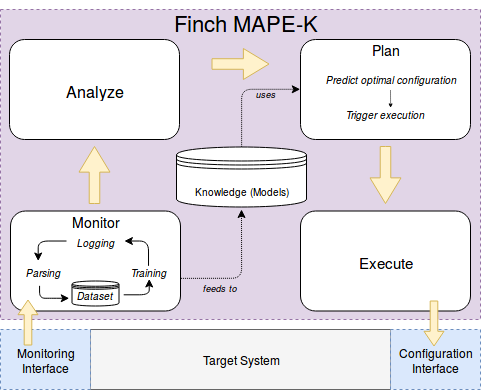
\includegraphics[scale=0.5]{images/FinchMAPE.png}
  \caption{\projectname{}'s ML-based MAPE-K feedback loop design. The knowledge base is composed of learned models. The monitor and plan components use machine learning techniques in order to build the dataset and create adaptation plans.}
  \label{fig:finchMape}
\end{figure}

These two Goroutines running in loop compose the main abstraction of \projectname{}: the MAPE-K feedback loop.

They communicate internally using Go's channels, which can be thought as pipes that connect concurrent Goroutines. The philosophy behind Go's channel is: share by communicating, not by sharing. Instead of sharing memory between threads, the sharing happens by sending messages between channels.
Instead of handling concurrency by using mutex locks, it's favored by Go's community to use channels and messaging. The main loop spawns two other goroutines and control them with two different channels.

The goroutine that periodically builds the dataset starts an inner loop that extract all metrics from Prometheus and builds the necessary dataset for training every $DatasetBuilderFrequency$ minutes as shown below, where this $DatasetBuilderFrequency$ is configurable.

Monitoring and analyzing the current context and state of the target system requires more non-trivial work, such as periodically extracting, from Prometheus, a single row of metrics of that given timestamp, analyzing, extracting, and saving the current state of all SLAs defined by the user for the target system against the current context, checking if there is any SLA violation, triggering the adaptation procedure, waiting for the adaptation to fully propagate, and checking for improvements in order to prevent unnecessary new adaptations.

Internally, \projectname{} implements a state machine to keep track of its operations in order to ensure that the target system is progressing and to control adaptations. Figure \ref{fig:statemachine} illustrates this state machine.

\begin{figure}[ht]
  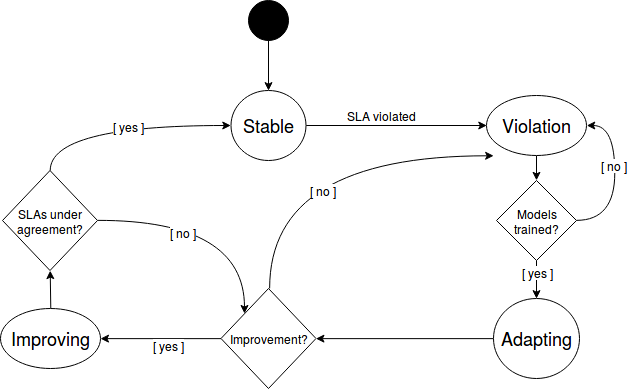
\includegraphics[width=\columnwidth]{images/FinchStateMachine2.png}
  \caption{\projectname{}'s state machine to ensure progress in the target system}
  \label{fig:statemachine}
\end{figure}

\subsection{Machine learning architecture}

Given the previously defined dataset, \projectname{} trains many different models, one for each SLA's indicator. In the end we want to predict the SLI, given the set of configuration parameters and system metrics---including workload. 

\projectname{} has 2 ML pipelines. The first one is training the models, which includes basic standardization, normalization, grid search, and cross validation. The Second one is predicting the SLI, given the configuration parameters. After running these pipelines, the last step is finding the optimal set of configuration parameters.

\subsubsection{Training pipeline}

As mentioned before, \projectname{} trains a model for each SLA indicator. To elaborate further on it;  if the user has two SLAs with respect to the latency of endpoint $A$ and $B$, then the two collected SLIs are the 99$^{th}$ percentiles of these endpoints' latency. Thus, \projectname{} will train two models, one for each SLI.

Training different models requires slicing the original dataset to fit the models' needs. For example, when we want to predict the latency of endpoint $A$, latency $A$ is the target, or $y$, of the model, and the corpus, or $X$, is the rest of the dataset \textit{minus} the other SLIs collected. This way, the system metrics, workload and configuration parameters are isolated for the model training.

\subsubsection{Learning how to learn: creating adaptive machine learning models}

Since the dataset is very personalized with respect to the target system, there's no one model to rule them all, for example: we cannnot simply use logistic regression or a neural network with static hyperparameters. A personalized dataset means that it can have an arbitrary dimension (number of features) and size, it can have only continuous values or discrete values, or both. \projectname{} cannot know this beforehand. Thus, to work with uncertain datasets, when training the models we must perform grid search.

Grid search is a technique to search for the best hyperparameters and models. Hyperparameters are parameters that are not directly learned by the models, parameters that configure certain aspects of a given machine learning models, for instance: how deep a decision tree should be, how many decision trees (i.e estimators) a random forest should have, or how many layers a neural network should have. Each machine learning model performs better when choosing the right model and the right hyperparameters for a given dataset. Some models-hyperparameters combination perform better with highly dimensional dataset, some perform better with well-balanced dataset, some are more resistant to outliers, sometimes the outliers is what you are trying to find. 

Given all these options and uncertainties with respect to the collected dataset, grid search is a way to find the most well suited model and hyperparameters for the dataset being collected by the target system.

Grid search exhaustively considers all hyperparameter combinations and many different models, train one model per combination, and select the most best performing one. This adds a considerate time and space complexity in the training pipeline, but it is something that cannot be avoided when choosing a model that will not overfit or underfit on dynamically generated datasets. 

However, the grid search is only performed in two scenarios: first training cycle, where \projectname{} first handles the extracted dataset, after the first training cycle, it will know the best hyperparameters for the learned models and use them to re-train the model with the new data. The second scenario where grid search is performed is when the model's prediction performance starts to degrade, meaning that the dataset changed in some aspects, thus, needing to re-learn better a model and hyperparameters for the new dataset.

In this pipeline, it is considered models such as linear regression, ridge regression, lasso, support vector machines, and decision trees. However, in the evaluations performed in this work, which used a few variations of dataset structure, we have found that one machine learning model/technique worked best the majority of times: gradient boosting with decision trees. 

Gradient boosting is not exactly a machine learning model, but rather a class of techniques called Ensemble, where instead of using a single model, we train many slightly different models with different portions of the dataset, and combine them in a variety of ways to achieve a higher performance. Unlike common and more simple ensemble techniques such as bagging. the trained models are not working independently, instead, they work sequentially in such a way that the following predictors learn from the mistakes of the previous predictors.

To validate the grid search and avoid overfitting, \projectname{} performs cross-validation with 5 splits, and $30\%\slash70\%$ test/train split ratio.

\subsubsection{Predicting the optimal configuration}

The user, when defining the adaptive configuration parameters, also defines the value range or the possible values, in case of discrete configuration parameters. For instance, a certain configuration parameter $A$ could take values ranging from $1$ to $100$, and another parameter $B$ could take the following array of discrete values: 1, 5, 10, 50.

After the models have been trained, we could simply predict the optimal configuration by passing the desired SLIs as our $X$, and in return get the optimal configuration as the $y$ coming from the prediction method.

However, that showed not to be very effective, and we devised an additional algorithm on top of this straightforward call to prediction method. This algorithm came as answer to cope with the following problem: in some cases, a configuration parameter does not overlap with respect to its effects on different SLAs, thus, in these cases, a model for a specific SLA predicts the right configuration parameter, but only for that given parameter which affects it directly, and makes inaccurate predictions for the other configuration parameters, since it does not affect it directly. This prediction affects other SLAs negatively. Think of an SLA being selfish and only caring about the configuration parameter that affects it, and not thinking about the other SLAs.

To overcome this problem and find the configuration that satisfies all SLAs or the majority of the SLAs, the algorithm created establishes some sort of consensus between the SLAs through a voting mechanism. To start it, it creates a 2D array with the Cartesian product of all possible parameter combinations, then, for each SLA, it predicts its respective SLI value for each of these combinations. The time to predict all these combinations is negligible, since predictions usually take a short amount of time, even with big matrices (show this in experiment).

Then, for each SLA's predictions, it filters the configurations that satisfy the SLA plus a tolerance rate. Now we have, for each SLA, a set of configuration that is both diverse and satisfiable. In the last step, for each configuration parameter, in case of a discrete parameter, we pick the one with the highest occurrence, and in case of a continuous value, we compute the mean of the predicted values for this parameter.

In the end it outputs the set of configuration parameters that, based on past experience, is most likely to satisfy all SLAs or the majority of SLAs.

\subsection{Passive and active training mode}

\projectname{} is always re-training its models with current data. However, the initial training cycles require grid search to be performed, and during these first few cycles, \projectname{} sits passively collecting data and training models, but not making predictions and adaptation plans. Thus, during this period, it is necessary to collect a diverse dataset, \projectname{} needs to know how to target systems respond to different configurations under different workloads. There are two ways to achieve that: passive and active training modes. These two options mode can be configured in \projectname{}'s configuration file. The passive mode just collects data and train models while the system is running, not intervening with the target system's natural flow. The active training mode, as a way to speed up the learning process, \projectname{} will actively and frequently mutate the configuration parameters in the target system in order to fasten the process of gathering a more diverse dataset.

% \subsubsection{Passive training mode}

% In passive training mode, \projectname{} will just collect data and train models while the system is running, not intervening with the target system's natural flow. Thus, this could mean taking a longer time for \projectname{} to start making adaptation plans, since it needs a diverse dataset. 

% \subsubsection{Active training mode}

% In active training mode, as a way to speed up the learning process, \projectname{} will actively and frequently mutate the configuration parameters in the target system in order to fasten the process of gathering a more diverse dataset. Thus, it will know sooner how the target system respond to different configuration settings. Running it alongside a workload simulator also works well, which is what we did to evaluate an experiment. Since this a risky move to make in production, \projectname{} should be ran alongside a testing/staging environment.


\section{Evaluation}

To guide and evaluate our work, four research questions are used:

\begin{itemize}
  \item \textbf{RQ1:} Can \projectname{} learn the optimal or sub-optimal configuration parameters in a target system?
  \item \textbf{RQ2:} How much performance overhead is incurred by \st{using} \projectname{}?
  \item \textbf{RQ3:} How much training data is needed to make accurate plans?
\end{itemize}

In the next subsection we discuss the setup for the experiment of the tool and techniques previously discussed.

\subsection{Experiment}

We needed a production level web service exposed over a REST API. It is very hard to find these as open source, and the ones that we found were usually a simple proof of concept for a tool. They mostly had very few endpoints and a simple business logic, which is not realistic enough to test \projectname{}. As a result, we developed a web service with this goal in mind. This system captured the most common points of complexity in web services, which are:

\begin{itemize}
  \item A backend component that holds all the core logic of the application and containerized with Docker.
  \item Multiple HTTP endpoints served over REST API. In our scenario, these endpoints are subject to a set of Service Level Agreements measured using APDEX. For instance, \textit{endpoint\_A\_POST} is an HTTP POST endpoint for the service $A$, and $X\%$ of all requests to it should not take more than $Y ms$ to respond.
  \item Another Docker container holding a Postgres database
\end{itemize}

At last, after developing this target system, small modifications on it were made in order to integrate \projectname{} into it, such as basic monitoring and providing SLAs file, adaptive configuration files, and adaptation methods.

\subsubsection{Initial training phase with workload simulation}


We found that, to make accurate and useful predictions, \projectname{} needed a dataset of reasonable size. However, my web service was not a system in production, and the only way to collect the mentioned dataset was through workload simulation. We accomplished this by mimicking realistic user cases for the system. For instance, a user can browse shopping items, add and remove  items arbitrarily to a shopping cart, and finalize the shopping session by checking out. The simulation we created ran these user cases multiple times in parallel in order to stress the system in a realistic way. 

At the end, \projectname{} ran alongside the target system for a while, collecting data and learning the system's patterns.


\subsubsection{Experiment 1: configuration-controlled throttling}

This first experiment intended to answer the following question: \emph{Can \projectname{} infer the optimal configuration parameters without being explicitly programmed?}

To validate and answer this initial question, we needed not to focus on implementation details of the actual configuration changing, for example, gracefully handling Docker's containers and Postgresql restarts.

To achieve this, we created a script that randomly (and temporarily) generates throttling points in the target system, these blocking points block the flow in the code for either $B_i$ milliseconds or $(\frac{1}{B_i}) * 10000$ milliseconds for each throttling point $B \in 1 \dots i$. That means that a throttling will block the flow either proportionally or inversely proportionally to the value of a configuration parameter. For instance, if a configuration value is $1000$, in a proportional throttle point, it will block the flow for 1000ms or 1s. In a inversely proportional throttle point, it will block the flow for 10ms. Thus, if this configuration can take a number between $1$ and $1000$, it could be one extreme or the other, depending on the type of throttling point.

These $B_i$ values are now our artificial configuration parameters that affect the performance of the target system. Thus, if \projectname{} can perform its workflow---monitor, analyze, predict, and execute the adaptation plan---and correctly create an adaptation plan and configure the parameters in such a way that the performance will be either optimal or sub-optimal, again, \emph{without being explicitly programmed for this task}, then we validate the architecture of \projectname{} is achieving its goals and that predicting real configuration parameters is a matter of dataset quality, and thus, time to learn correctly.

We ran 3 different sets of random artificially generated configuration parameters and studied \projectname{}'s performance on them. We focused on 3 questions during this experiment:

\begin{itemize}
  \item Can \projectname{} predict the optimal or the sub-optimal configuration?
  \item If yes, how long does it take to converge to the optimal or sub-optimal configuration?
  \item How accurate is the model?
\end{itemize}

For the model accuracy, it was used the coefficient of determination $R^2$ of the prediction, where $R^2 = 1 - \frac{u}{v}$, where $u$ is the residual sum of the squares  $\sum_{i=1}^{n}(y_{true} - y_{pred})^2$ and $v$ is the regression sum of squares $\sum_{i=1}^{n}(y_{true} - \overline{y_{true}})^2$.

\subsubsection{Experiment 1 results}

All tests were ran on a personal Dell laptop running Ubuntu 14.04 with 4 Intel Core i7-5500U CPU @ 2.40GHz and 16 GB of memory ram. The machine learning code makes uses of parallelism on all 4 cores when training the models and predicting.

Each training cycle equals 1 hour, the target system had 5 configuration parameters. From these experiments it is possible to see that after the first cycle \projectname{} learns to find the optimal set of configuration parameters, achieving 100\% on its predictions and stabilizing after the second cycle. Table \ref{tab:experiment1} shows the results of these 3 experiments.

Training cycle can become a bottleneck if we keep growing the dataset for many days, however this is an easy bottleneck to overcome, as the user can configure \projectname{} to extract the dataset less frequently after it gets a stable model accuracy. For future work, training the models could be easily distributed to machines that are not running the target system, in order to prevent resource saturation and affect the service quality.

Predicting the optimal configuration parameters is surprisingly fast, performing the prediction around 100 milliseconds and 200 milliseconds, even with the algorithm to find the best optimal configuration by performing multiple exhaustive predictions.

For all three runs of the experiment, after the second training cycle, it took between 5 to 10 minutes for the target system stabilizes all its SLA violations.

\begin{table*}[t]
\caption{Data from using \projectname{} with artificially generated configuration parameters}
\label{tab:experiment1}
\begin{tabular}{llllll}
\hline
Run 1     & Configuration precision & Models average accuracy & Dataset size (\# of rows) & Training time    & Prediction time  \\ \hline
Initial   & 40\%                    & N.A                     & N.A                       & N.A              & N.A              \\
Cycle \#1 & 60\%                    & 71\%                    & 326                       & 46 seconds       & 200 milliseconds \\
Cycle \#2 & 100\%                   & 80\%                    & 1082                      & 1 min 20 seconds & 117 milliseconds \\ \hline
Run 2     & Configuration precision & Models average accuracy & Dataset size (\# of rows) & Training time    & Prediction time  \\ \hline
Initial   & 40\%                    & N.A                     & N.A                       & N.A              & N.A              \\
Cycle \#1 & 60\%                    & 68\%                    & 374                       & 51 seconds       & 165 milliseconds \\
Cycle \#2 & 100\%                   & 80\%                    & 1165                      & 1 min 12 seconds & 128 milliseconds \\ \hline
Run 3     & Configuration precision & Models average accuracy & Dataset size (\# of rows) & Training time    & Prediction time  \\ \hline
Initial   & 20\%                    & N.A                     & N.A                       & N.A              & N.A              \\
Cycle \#1 & 80\%                    & 87\%                    & 334                       & 43 seconds       & 125 milliseconds \\
Cycle \#2 & 100\%                   & 94\%                    & 1125                      & 1 min 7 seconds  & 119 milliseconds
\end{tabular}
\end{table*}


\subsubsection{Experiment 2: performance overhead evaluation}

Given the results found in experiment 1, the training algorithm is observed to become a bottleneck as the dataset gets bigger. To investigate this bottleneck further and to closely observe \projectname{}'s resouce usage, we collected a bigger dataset, with a total of 28147 rows and for 10 hours. The strategy for the configuration parameters used were the same as in the first experiment; random throttling points in the target system's code.

The first training cycle, the one that performs an expensive grid search, took 29 minutes to find the optimal models and their hyperparameters for 5 SLI models. The subsequent training already knew the best model( so it just fitted the model onto the data), and took 4 minutes to train and 268 milliseconds to predict.

\subsubsection{How much performance overhead is incurred by \projectname{} and Prometheus}

Golang's pprof was used to perform a thorough profiling of both CPU-time and heap of the target system when using \projectname{}.

While acting as a passive co-pilot (no training and no adaptations created/carried out) and monitoring alongside Prometheus, \projectname{}'s performance overhead over a 2-minute profiling window was 90 milliseconds out of 1530 milliseconds (5.88\%). In this 2-minute window, Finch's MAPE-K loop, its main component, took 40 milliseconds out of 1530 milliseconds (2.61\%), as shown in figure \ref{fig:mapeoverhead}. Thus, while running only its monitoring/analyzing loop, \projectname{} incurred roughly 8.5\% CPU overhead. This answers the second research question (\textbf{RQ2})


\subsubsection{Experiment 3: finding the optimal configuration for Postgres}

It is known that, because of the fact that Postgres contains a very big set of configuration parameters, it is a challenging task to adapt Postgres to different scenarios. For instance, for a certain type of query, properly configuring Postgres' \textit{work\_memory} variable can drastically improve its performance. There are many cases like this one, however, it would not be productive to discuss each one of them.

In this example, we use \projectname{} in the same target system from experiment 1 and 2, but now instead of random throttling points, \projectname{} tries to learn how to better configure the Postgres database behind the target system.

Postgres $9.4$ was used, and the monitored configuration parameters were:

\begin{itemize}
  \item Shared buffers
  \item Effective cache size
  \item Work memory
  \item Write ahead log (WAL) buffers
  \item Checkpoint completion target
  \item Maintenance work memory
  \item Checkpoint segmnets
  \item Default statistics target
  \item Random page cost
\end{itemize}

The SLAs were the same as in the previous experiments. However, the adaptive configuration file is different, as it contains all previously cited Postgres parameters and in each one of them, it defines the configuration parameter as a custom one, pointing it to the appropriate file that contains a procedure that \projectname{} should run when adapting this configuration parameter, as shown in listing \ref{lst:adaptiveconfig1}.

The adaptive method in this experiment, called \emph{configurePG}, takes the predicted optimal configuration and perform the following actions:

\begin{itemize}
\item Loads the current Postgres configuration file.
\item Changes the predicted parameters to their respective predicted values and persists it to disk.
\item Using Docker remote API, it creates a new Postgres container, which loads the new configuration file, this Postgres instance points to the same volume as the current running Postgres instance.
\item Tells the service what is the new Postgres instance's ip:port.
\item Kills the previous Postgres Docker container
\end{itemize}

This way, all changes to Postgres will be effective because of the full restart of the instance.

\begin{lstlisting}[float,floatplacement=H,caption={Example of one of the adaptive configurations used in experiment 3},label={lst:adaptiveconfig1}]
[
  "pg_shared_buffers": {
    "value": 128,
    "valueType": "discrete",
    "values": [16, 128, 4000, 16000],
    "isCustom": true,
    "adaptationMethod": "configurePG"
  }
]
\end{lstlisting}

\subsubsection{Results}

In this experiment, the target system started with the default configuration for Postgres. After a while, given the heavy workload, some of the SLAs were violated. However, that happened before \projectname{} learned its models, so nothing could be done before the training. After the training cycle, which took 2 hours, \projectname{} triggered an adaptation, since the target system was in a state of SLA violation. After predicting the best optimal configuration for that scenario and carrying out the adaptation, the 99th percentile latency was reduced by $39.85\%$, the comparison of before and after the adaptation can be seen in figure \ref{fig:pgexperiment}. Thus, answering the research question 1 (\textbf{RQ1}).

\begin{figure}[!ht]
	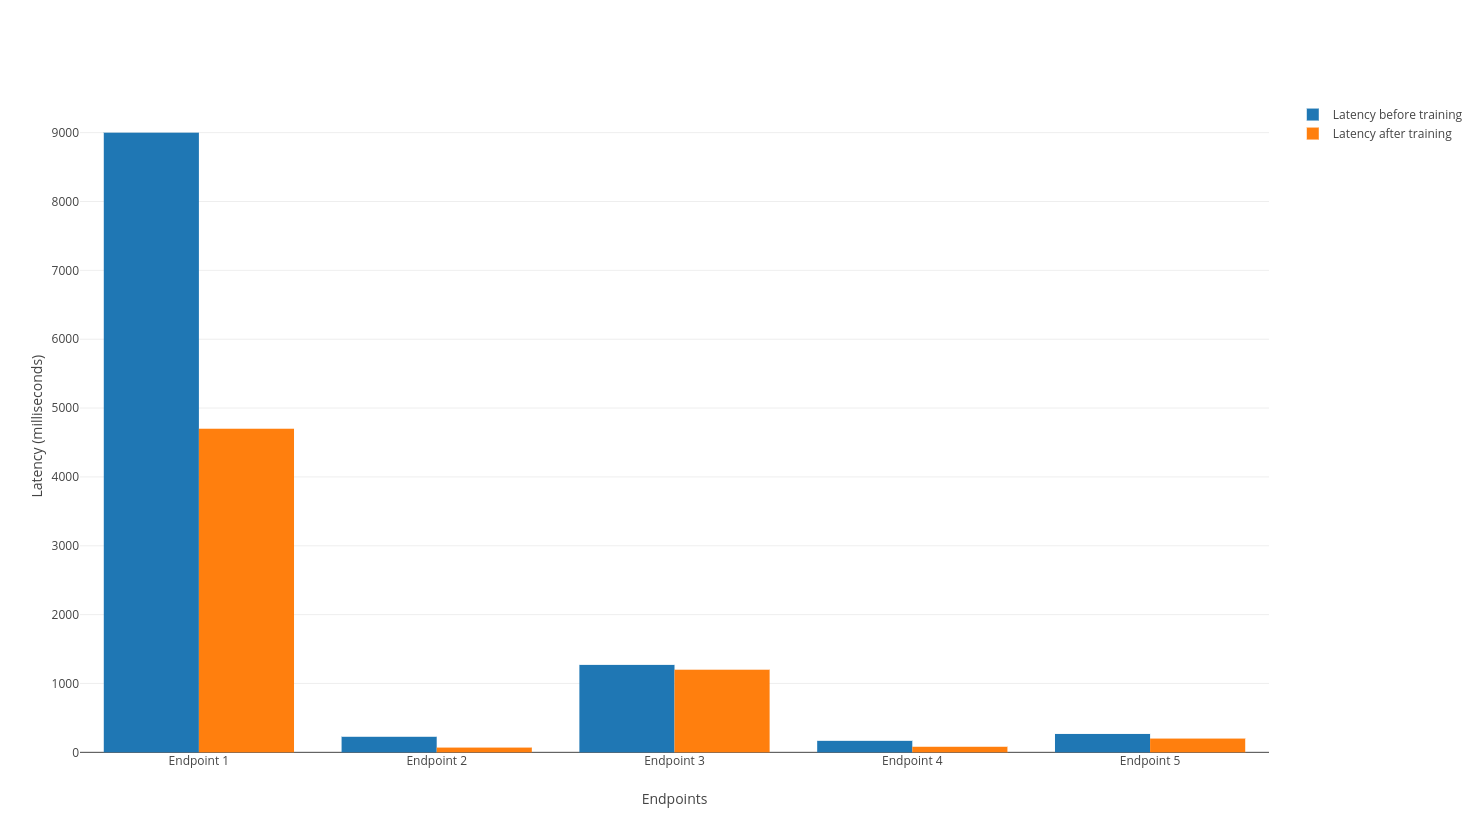
\includegraphics[scale=0.15]{images/pgexperiment.png}
  \caption{Experiment 3: 99th percentile latency of all endpoints before and after adaptation. Each item in the X axis is an endpoint affected by a configuration parameter. Y axis is the latency. The average latency reduction was $39.85\%$.}
  \label{fig:pgexperiment}  
\end{figure}

\subsubsection{How much data is needed to make accurate predictions?}

The research question 3 (\textbf{RQ3}) touches a question commonly asked in the machine learning community: how much data is needed to make accurate predictions?

The answer to this question is: it depends on the properties of the dataset, such as size (how many rows), dimension (how many features), and overall quality of the dataset. For both experiments 1 and 3, it was needed at least 1000 rows in the dataset to reach a good cross validation accuracy. However, this could change if we had many more configuration parameters.

This brings up an important takeaway point from this work: the empirical knowledge collected from running Finch in one target system will not properly transfer to running Finch in a different target system with different contexts and components. Even thought that is the case, Finch was designed to handle this uncertainty, as its training pipeline performs an extensive grid search to find the best model for a given observed dataset.


\section{Discussion and future work}

As of now, \projectname{} is in its initial version and it is highly experimental. Thus, it has some limitations that should be addressed by future improvements.

The main additional overhead that comes with \projectname{} is due to using Prometheus for storing observed data. To address the Prometheus performance overhead, a simple time-series database to store its logged events is enough for \projectname{}. Such a database could be implemented from scratch as a simple log storage, or by using TimescaleDB, a simple implementation of time-series constructs on top of Postgres.

In some training cycles, grid search is automatically used in order to improve the quality of the accuracy. This special and costly training happens during the first few cycles, and when the accuracy starts dropping, usually because of change in the usage patterns.

Because this is a very computationally expensive operation, this can negatively affect the target system by using too much compute power during the training operation. This performance issue could be solved by distributing this training pipeline to other machines or simply delegating the training to an external service will solve the problem.

To address the lack of a control interface, a web UI that talks directly to \projectname{} over a REST API should be implemented. Such UI should provide control over \projectname{} 's workflow.


\section{Conclusions}
This work presented Finch; a tool that was designed to enable self-adaptation in systems without requiring complex architectural changes. As of now, the tooling for building self-adaptive systems is very scarce and complex in the software industry. We propose Finch as a step in the direction to build tools that make it possible to enable configuration self-adaptation in non-autonomous systems.

We show that Finch learns how to properly configure a target system after it ran alongside the system for a while. Once Finch is imported into a system, it starts collecting data on the context of the system. When the workload pattern changes or the performance of the system degrades, Finch executes adaptations that change the system’s configurations, which successfully optimizes the system's performance. The success of the adaptation stems from the machine learning-based MAPE-K feedback loop that is injected into the target system. As a result, besides enabling configuration self-adaptation in systems, Finch also addresses the complexity of configuring software systems that have a high degree of uncertainty in their environment.

As the goal of Finch is to make integration to systems easier, it also provides a small and concise API, and incurs a performance overhead no higher than 8.5\%. 

For future work, we discuss how the design of Finch can be improved in order to decrease its performance overhead, and make setting up Finch easier. The principle behind this work is that, rather than having hard-wired heuristics, systems should be able to adapt to different usage patterns by changing aspects of itself.
%\end{document}  % This is where a 'short' article might terminate

% \nocite{*}

%\begin{acks}

%\end{acks} 